\chapter{Tecnologie di sviluppo del front-end}
\label{chap:tecnologie di sviluppo del frontend}

Per rendere lo sviluppo della dashboard più rapido e fluido si è deciso di adottare un framework web. La scelta è ricaduta sulla libreria ReactJS e sull'ottima integrazione con Redux che ha permesso più semplice l'organizzazione e il riutilizzo del codice.

\section{React}
\label{sec:react}

React è una libreria JavaScript per lo sviluppo di interfacce sviluppata da Facebook Inc. e rilasciata pubblicamente nel giugno 2013.
Secondo la definizione ufficiale data dai suoi stessi sviluppatori, React è una singola libreria interamente focalizzata alla realizzazione di interfacce grafiche. La forza di React rispetto ad altre librerie è quella di consentire l’uso di un approccio dichiarativo simile alla sintassi HTML, quindi molto familiare, per definire i componenti che rappresentano parti significative e logiche dell’interfaccia utente, ad esempio un commento a un articolo, o la lista degli stessi commenti.
Nonostante React sia stata inizialmente sviluppata per essere eseguita sul DOM di un browser moderno, la sua architettura le consente di funzionare in ambienti differenti,
come ad esempio un'applicazione web o anche come software nativo sui sistemi operativi Android e iOS. Infatti la libreria si occupa di manipolare un'interfaccia grafica a partire da
un insieme di dati che ne descrivono la struttura ed il comportamento, astraendo tutto ciò
dall’ambiente in cui verrà effettuato il rendering finale.
Nel corso di questa trattazione, verrà utilizzata come versione di riferimento la 16.8 di
React.

\subsection{Componenti}
\label{sec:componenti}

React ha un'architettura fortemente orientata ai componenti. Per componente si intende una porzione di interfaccia che deve essere considerata come un'unità a sé stante, in grado di gestire una propria logica interna e pensata per poter essere riutilizzata ovunque venga richiesta una funzionalità simile. Una porzione di interfaccia più complessa si potrà ottenere tramite l’utilizzo di uno o più componenti di base, che potranno mutare il loro aspetto
a seconda del contesto in cui vengono collocati.
In React ogni componente può essere considerato come una funzione: come argomento accetta un insieme arbitrario di dati, utili per determinare come apparirà e si comporterà il componente, e come risultato si otterrà una rappresentazione grafica del componente, come ad esempio un elemento del DOM.
Ci sono due modi diversi con cui è possibile combinare i componenti e i dati: sia \textit{props} o \textit{state}. Questi due oggetti determinano ciò che esegue il rendering di un componente e come si comporta.
I dati ricevuti in input in React sono denominati \textit{prop}. \textit{State}, d'altra parte, è un oggetto che è di proprietà del componente dov'è dichiarato. Il suo ambito di applicazione è limitato al componente corrente. Un componente può inizializzare il proprio state e aggiornarlo ogni volta che è necessario. Lo state del componente genitore solitamente finisce per essere il \textit{props} del componente figlio. Il compito di rappresentare graficamente il componente è demandato alla funzione render() del componente.

Il codice sottostante riporta un esempio molto semplice di componente React: ad esso viene passato un valore \textit{name} tramite \textit{props} che viene stampato a video con l'elemento titolo \textit{h1} ritornato dalla funzione render().

\lstinputlisting[style=JavaScriptStyle]{code/componentExample.js}

L'esempio appena riportato mostra il componente Welcome rappresentato come \textit{componente di classe}. React offre la possibilità di definire i componenti come semplici funzioni JavaScript e, con l'integrazione a ES6, come funzioni arrow. Questa scelta porta vantaggi e svantaggi: da un lato offre la possibilità di scrivere un codice più pulito e avere una sintassi concisa, ma dall'altro non è possibile definire lo \textit{state}. In questi due casi si può parlare anche di componenti Stateful (componenti di classe) e componenti Stateless (componenti di funzione). 

\lstinputlisting[style=JavaScriptStyle]{code/functionComponentExample.js}

Per lo sviluppo della dashboard ho adottato nella maggior parte casi la definizione dei componenti mediante funzioni arrow, utilizzando gli hook di React per gestire i vari stati (questo argomento viene trattato nei seguenti paragrafi).

\subsection{JSX}
\label{sec:jsx}

Un altro elemento che rende la sintassi dei componenti più chiara e comprensibile è JSX. JavaScript eXtension, o più comunemente JSX, un’estensione della sintassi JavaScript che consente di scrivere tag ed elementi HTML all'interno di porzioni di codice JavaScript. React non obbliga ad utilizzare JSX, ma la maggior parte delle persone lo trovano utile come aiuto visuale quando lavorano con la UI all'interno del codice JavaScript. Dopo la compilazione, le espressioni JSX diventano normali chiamate a funzioni JavaScript che producono oggetti JavaScript.

In basso sono riportati due esempi: il primo riporta un componente React definito senza l'utilizzo di JSX, mentre il secondo è implementato con l'ausilio di JSX.

\lstinputlisting[style=JavaScriptStyle]{code/NoJSXExample.js}

\lstinputlisting[style=JavaScriptStyle]{code/JSXExample.js}

Si può notare immediatamente come il codice, nel secondo caso, risulta più intuitivo e leggibile. Inoltre, permette di evitare l'utilizzo della funzione \textit{React.createElement} per ogni elemento che occorre definire. 
All'interno tag JSX è possibile inserire qualsiasi espressione JavaScript all'interno delle parentesi graffe. Considerando la riga 3 dell'esempio che adotta JSX, si osserva la dichiarazione di contenitore \textit{<div>} contente l'espressione JavaScript \textit{this.props.toWhat}. Ad ogni aggiornamento della variabile passata al componente tramite \textit{props}, viene eseguito un nuovo render che mostra il nuovo valore dell'espressione fra parentesi graffe.

\subsection{Ciclo di vita di un componente}
\label{sec:ciclo di vita di un componente}

Ogni componente React è caratterizzato da un ciclo di vita. All'interno dei componenti di classe è possibile definire dei metodi particolari (\textit{lifecycle hooks}) che si possono utilizzare per intercettare alcuni istanti del ciclo di vita di un componente e stabilire un determinato comportamento per quel componente. Per esempio, è possibile far eseguire determinate azioni quando un componente viene creato, aggiornato o distrutto o, addirittura, decidere se un componente deve essere modificato in seguito alla variazione di almeno una delle proprietà contenute nel suo oggetto State o alla ricezione di nuove \textit{Props}.
Nel ciclo di vita di un componente React possiamo distinguere essenzialmente tre fasi:
\begin{itemize}
    \item inizializzazione del componente
    \item aggiornamento del componente tramite la funzione \textit{setState} o la ricezione di nuove \textit{props}
    \item rimozione di un componente
\end{itemize}


\begin{figure}
\begin{center}
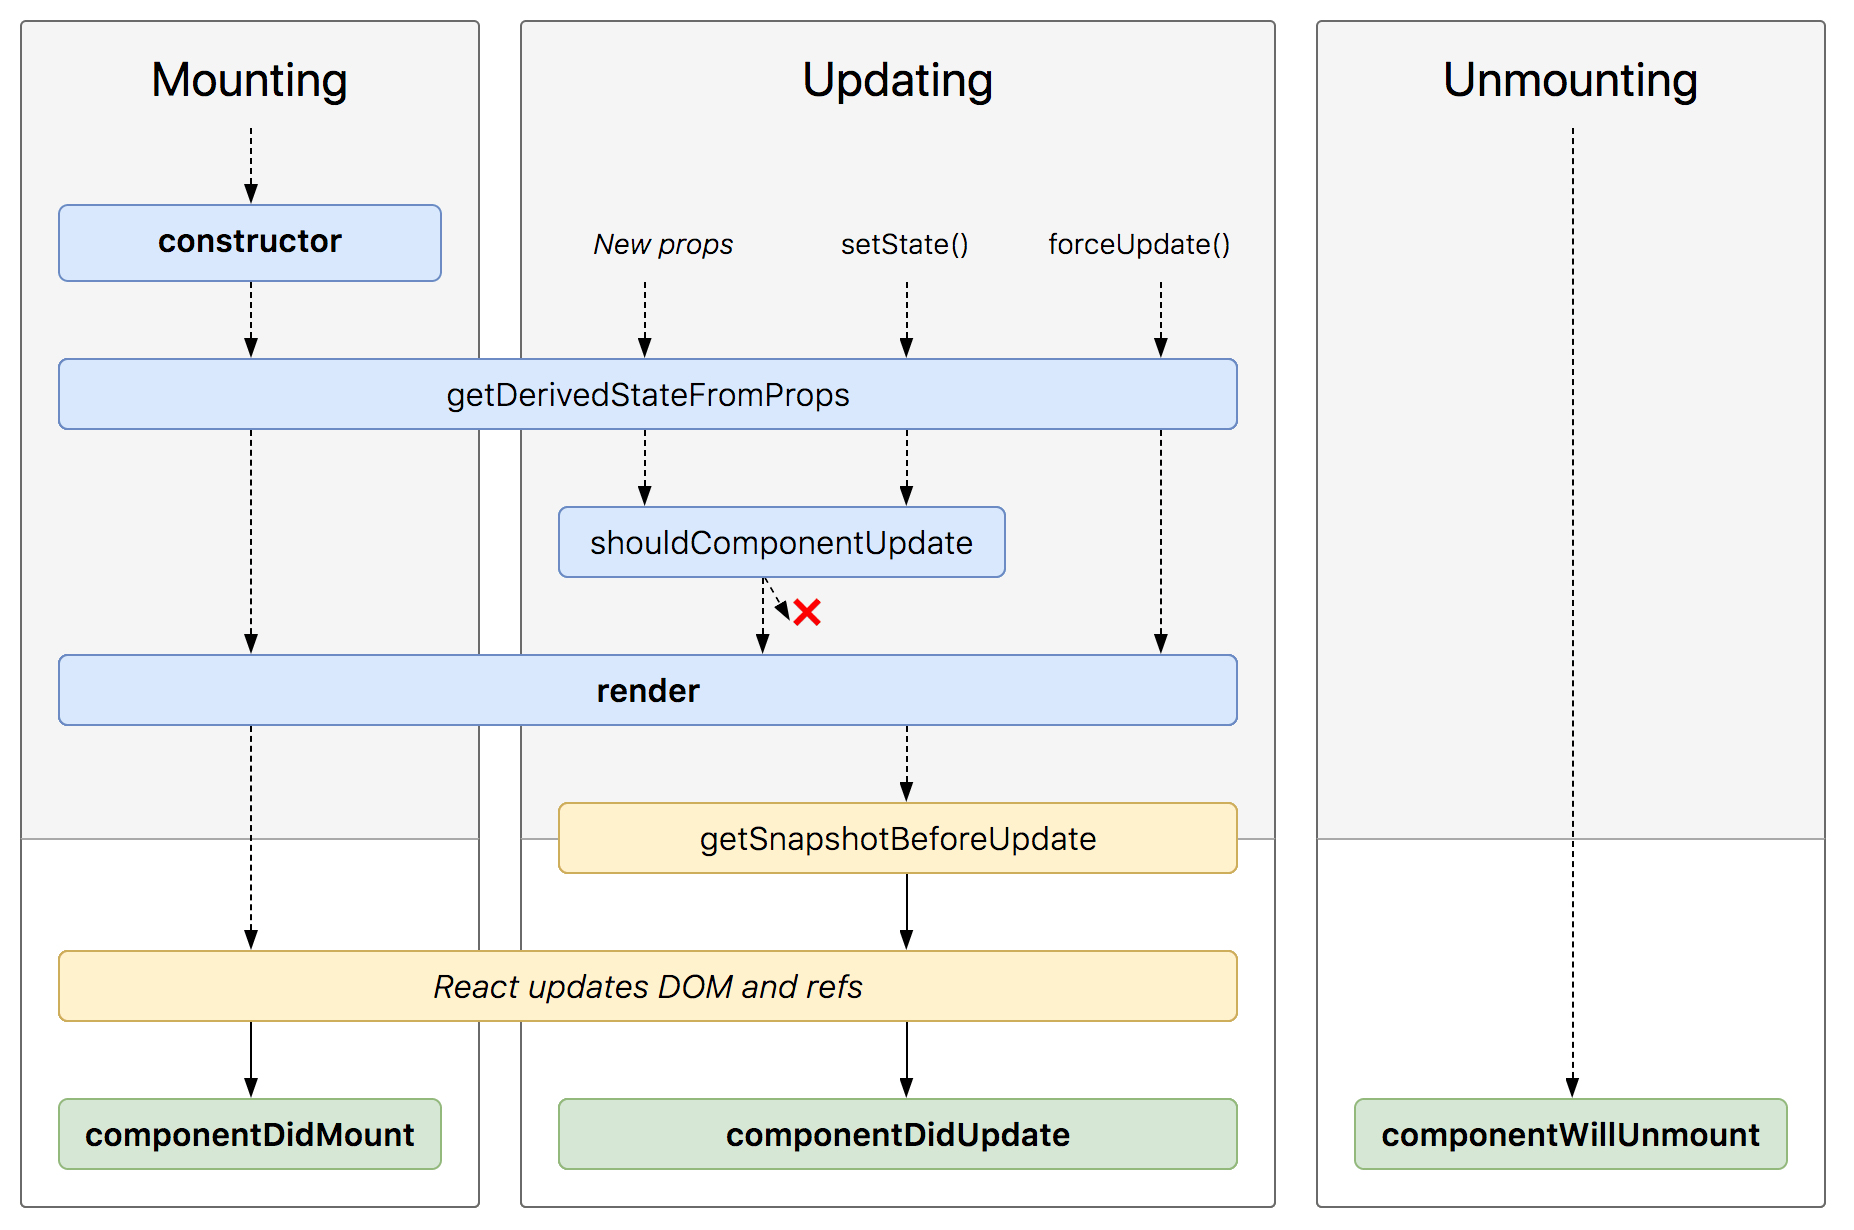
\includegraphics[scale=0.22]{main/images/lifecycleComponent.jpg}
\end{center}
\caption{Ciclo di vita di un componente.}
\label{fig:lifecycleComponent}
\end{figure}

Il costruttore è il primo metodo che viene chiamato. Per una corretta inizializzazione, all'interno del costruttore di un componente, dovremo innanzitutto invocare il costruttore della classe base \textit{super(props)} (come abbiamo visto definiamo un componente estendendo React.Component) passando le \textit{props} ricevute dal componente. 
Il secondo metodo ad essere invocato, immediatamente prima della funzione \textit{render()}, è \textit{componentWillMount()}. React consiglia di usare il costruttore al posto di questo metodo per ogni inizializzazione, poiché invocando la funzione \textit{setState()} all'interno di questo metodo gli altri \textit{licecycle hooks} non vengono richiamati.
La funzione \textit{render()} è l'unico metodo obbligatorio quando si vuole definire un componente. Non deve modificare direttamente l'oggetto \textit{props} o \textit{state}. All'interno della funzione render() non si deve manipolare il DOM o effettuare chiamate a funzioni per acquisire dati da un server. \textit{ComponentDidMount()} viene invocata dopo la funzione render(). Questo è il metodo da usare per manipolare il DOM o per recuperare eventuali dati da un server. Le valutazioni fatte in merito all'oggetto State nel metodo \textit{componentWillMount()} valgono anche per \textit{ComponentDidMount()}.

Quando viene aggiornato l'oggetto \textit{state} o in caso di ricezione di nuove \textit{props}, vengono invocati una serie di metodi in sequenza.
Il primo è \textit{shouldComponentUpdate()} che riceve come argomenti gli oggetti \textit{nextProps} e \textit{nextState} i quali rappresentano il prossimo valore dell'oggetto \textit{props} e dell'oggetto State. Il metodo \textit{shouldComponentUpdate()} restituisce un valore booleano. Se restituisce \textit{false}, i metodi successivi non verranno invocati. Di default questo metodo restituisce \textit{true}, consentendo l'aggiornamento del componente ad ogni modifica degli oggetti \textit{state} e \textit{props}. Per questo motivo, può essere usato per determinare se il componente deve essere aggiornato con i prossimi valori di \textit{props} e \textit{state}. All'interno di questo metodo è infatti possibile comparare i valori attuali degli oggetti \textit{state} e \textit{props} con quelli di \textit{nextState} e \textit{nextProps}, permettendo così di decidere se effettuare l'aggiornamento del componente, restituendo \textit{true} o \textit{false}.
Dopo il metodo render(), viene invocato \textit{componentDidUpdate()} che può essere usato per scaricare dati aggiornati da un server (nel caso per esempio ci sia stato un aggiornamento dell'oggetto \textit{props} o \textit{state}) o per operare sul DOM.

Nel fase di distruzione di un componente, invece, viene invocato come unico metodo \textit{componentWillUnmount()} che potremo usare per operazioni come invalidare eventuali timer avviati nella funzione \textit{componentDidMount()} e altre operazioni di manutenzione che prevengano memory leak.

\lstinputlisting[style=JavaScriptStyle]{main/code/lifecycleExample.js}

Il componente Clock nell'esempio imita il funzionamento di un orologio, mostrando a schermo la data
e l’ora corrente e aggiornandole ogni secondo. All’inizio del ciclo di vita del componente,
cioè quando questo viene montato per la prima volta nel DOM, viene richiamata la funzione \textit{componentDidMount()}, e il componente inizializza il proprio state, impostando
la data e l’ora.
Durante l’esecuzione di \textit{componentDidMount()} viene impostato un timer, che scatterà
ogni secondo fino a quando non viene fermato esplicitamente. Questo timer, ogni volta
che scatterà, chiamerà la funzione \textit{tick()} del componente. Questa funzione esegue a
sua volta un \textit{setState()}, e imposta anch’essa lo stato del componete con l’ora corrente.
Infine quando il componente viene rimosso dal DOM il timer viene fermato, in modo che
\textit{tick()} non venga più richiamato quando il componente verrà rimosso dal DOM e distrutto.

\subsection{Hooks}
\label{sec:hooks}

Gli Hooks sono stati aggiunti in React 16.8 e permettono di utilizzare \textit{state} ed altre funzioni di React senza dover scrivere un componente sottoforma di classe. Gli Hooks sono funzioni che ti permettono di “ancorarti” all’interno delle funzioni di React state e lifecycle da componenti funzione. 

Uno degli hooks fondamentali è \textit{useState}, un Hook che ti permette di aggiungere lo state React nei componenti funzione. L’unico argomento per l’Hook useState() è lo stato iniziale. A differenza delle classi, lo state non deve essere un oggetto. Possiamo tenere un numero o una stringa se è quello di cui abbiamo bisogno. La \textit{useState} ritorna una coppia di valori: lo stato corrente ed una funzione che lo aggiorna. Questi due valori vengono assegnati ad un array grazie alla sintassi JavaScrypt chiamata destrutturazione di array.

\lstinputlisting[style=JavaScriptStyle]{main/code/hookExample.js}

Grazie a \textit{useState()} ora è possibile definire componenti funzione con il proprio stato. L'unico grosso vantaggio che posseggono i componenti di classe sono i metodi lifecycle. Per ovviare a questa mancanza è stato introdotto l'hook \textit{useEffect()} che offre la possibilità di comportamenti simili alle funzioni \textit{componentDidMount()}, \textit{componentDidUpdate()} e \textit{componentWillUnmount()}.
L'hook \textit{useEffect()} accetta due argomenti: il primo argomento è una funzione callback che viene eseguita  dopo il render del componente; mentre il secondo argomento è un array di valori, solitamente corrispondenti alle \textit{props}. Se l'array non viene espresso la callback viene invocata dopo ogni render; quando l'array è presente ma non contiene alcun elemento la callback viene richiamata solo alla creazione del componente (\textit{componentDidMount()}). Se invece, l'array contiene dei valori, la funzione viene eseguita solamente alla variazione di almeno una delle variabili specificate in esso (\textit{componentDidUpdate()}). Se, come valore di ritorno della funzione di callback, viene definita una ulteriore funzione, questa viene eseguita appena prima della distruzione del componente imitando il ruolo del metodo \textit{componentWillUnmount()}.

Il codice riportato sotto riprende l'esempio mostrato nel paragrafo del ciclo di vita del componente, rivisto con l'utilizzo degli hook.

\lstinputlisting[style=JavaScriptStyle]{main/code/hookEffectExample.js}

\subsection{Routing}
\label{sec:routing}
Grazie all'utilizzo della libreria React è possibile sviluppare le cosiddette "single-page application", cioè applicazioni che si basano su una singola pagina HTML. Nel caso di React questo è possibile grazie al render di componenti diversi all'interno del medesimo elemento HTML, dando l'impressione all'utente di spostarsi in pagine differenti. 

Questo lavoro è agevolato dalla libreria React-router\footnote{React-router: \url{https://reacttraining.com/react-router/}} offrendo una collezione di API completa e semplice da usare. 

L'integrazione di questa libreria porta con sé vantaggi e svantaggi. La possibilità di creare una "single-page application" permette di evitare richieste HTTP al web server per ogni reindirizzamento di pagina, rendendo più fluida ed intuitiva la navigazione. Al contempo, la web application dev'essere caricata nella sua interezza ad ogni visita, anche se alcune pagine non vengono utilizzate. Questo può essere un grosso difetto per applicazioni web di grandi dimensioni poiché i tempi di caricamento iniziale si dilaterebbero notevolmente.

\subsection{Il pattern Flux}
\label{sec:flux}

Flux è l'architettura dell'applicazione che React utilizza per creare applicazioni Web sul lato client. Completa i componenti della UI di React utilizzando un flusso di dati unidirezionale.

Le applicazioni Flux hanno tre parti principali: il \textit{dispatcher}, gli \textit{store} e le \textit{view} (componenti React). Questi non devono essere confusi con le entità che compongono MVC (Model View Controller), pattern maggiormente diffuso per strutturazione di software che utilizza elementi grafici. I controller esistono in un'applicazione Flux, ma sono fortemente legati alle \textit{view}, cioè ai componenti React.

Flux evita gli standard del pattern MVC a favore di un flusso di dati unidirezionale. Questa scelta è dovuta al fatto che la maggior parte dei framework JavaScript, tra cui React, fornisce il supporto per l'associazione dei dati che consente alla vista di dialogare direttamente con il modello. L'adozione di MVC, quindi, renderebbe lo sviluppo e il debug di applicazioni di dimensioni importanti molto difficoltosa.
Quando un utente interagisce con una vista React, la vista propaga un'azione attraverso un \textit{dispatcher} centrale, ai vari \textit{store} che contengono i dati dell'applicazione e la logica di business. A sua volta aggiorna tutte le \textit{view} interessate. Funziona particolarmente bene con lo stile di programmazione dichiarativo di React, che consente all'archivio di inviare aggiornamenti senza specificare come passare da una vista all'altra.

\begin{figure}
\begin{center}
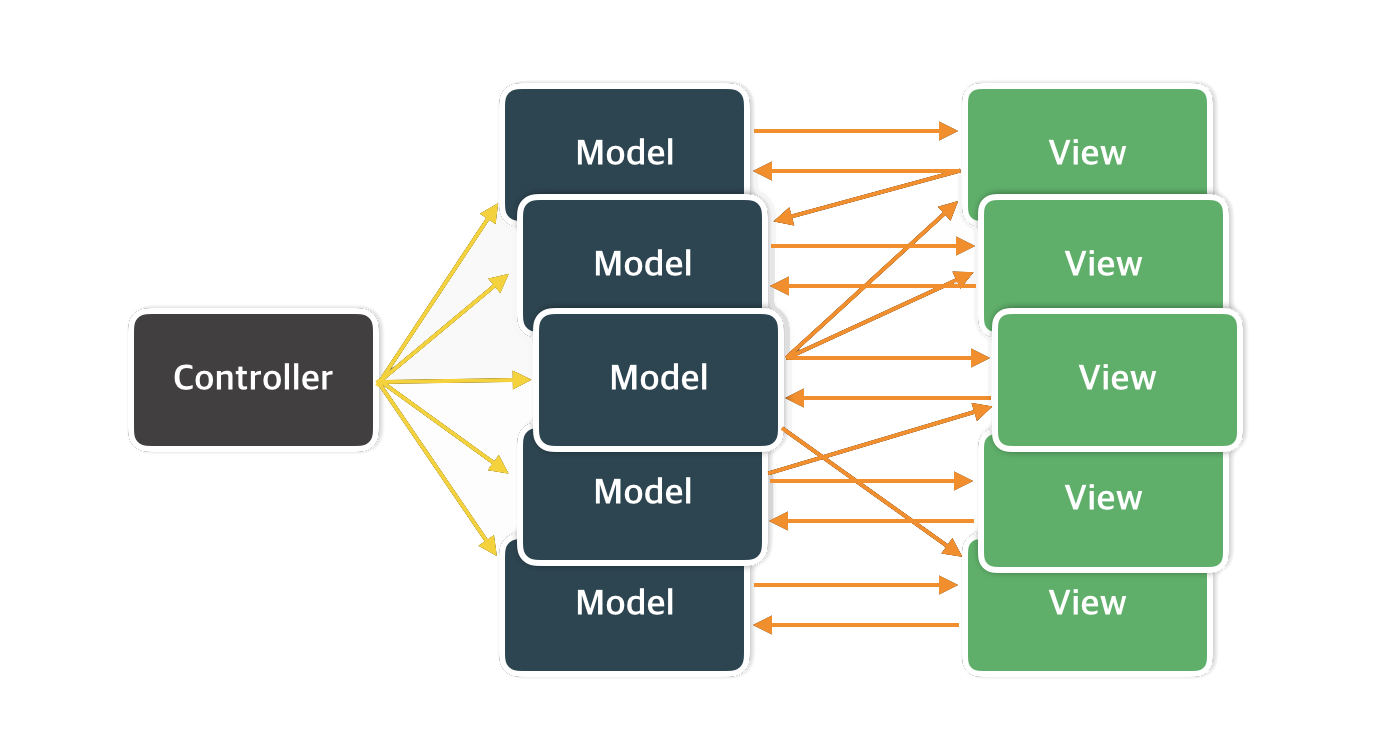
\includegraphics[scale=0.3]{main/images/mvc.png}
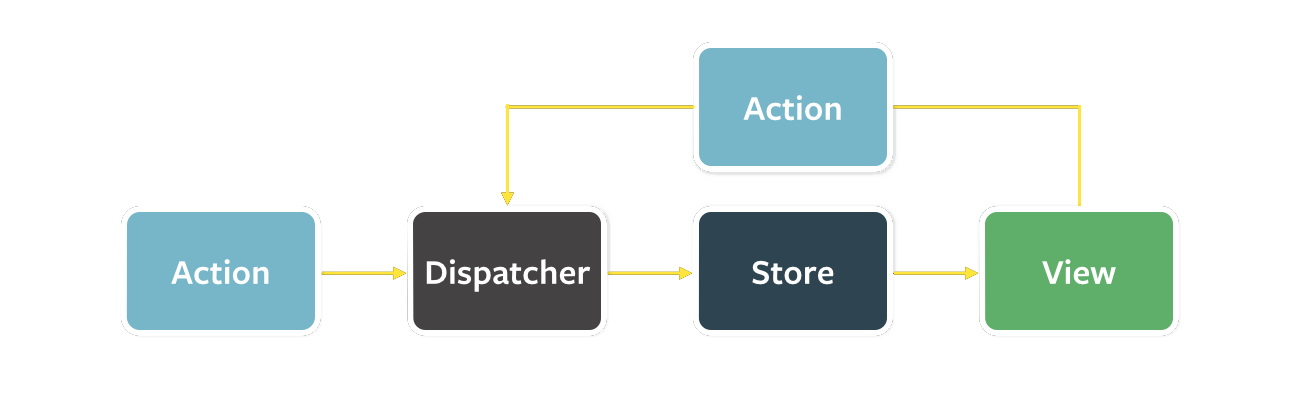
\includegraphics[scale=0.3]{main/images/flux.png}
\end{center}
\caption{Struttura del pattern MVC (in alto) e Struttura del pattern Flux (in basso).}
\label{fig:pattern}
\end{figure}

Un flusso di dati unidirezionale è fondamentale per il modello Flux. Il \textit{dispatcher}, i \textit{negozi} e le \textit{view} sono nodi indipendenti con input e output distinti. Le azioni sono oggetti JavaScript semplici contenenti i nuovi dati e una proprietà \textit{type} che identifica la tipologia dell'azione.

Le \textit{view} possono causare una nuova azione da propagare attraverso il sistema in risposta alle interazioni dell'utente. Tutti i dati passano attraverso il \textit{dispatcher} come un hub centrale.  Il \textit{dispatcher} quindi richiama le funzioni di callback che gli \textit{store} hanno registrato con esso. All'interno delle callback registrate, gli \textit{store} rispondono a qualsiasi azione rilevante per lo stato che contengono. Gli \textit{store} emettono quindi un evento di modifica per avvisare i componenti che si è verificata una modifica al livello dati. Le \textit{view} invocano il proprio metodo \textit{setState()}, causando un nuovo rendering di se stessi e di tutti i loro discendenti nella struttura dei componenti.

\subsection{Integrazione in OVL Dashboard}
\label{sec:integragrazione in OVL Dashboard}

Di seguito è riportata l'implementazione del componente \textit{ticket} di OVL Dashboard. È possibile notare l'utilizzo di svariati hook \textit{useState()} per tenere traccia di tutti gli aspetti di un ticket ed effettuare il re-render ad ogni loro cambiamento. Particolare, inoltre, è l'utilizzo di due differenti hook \textit{useEffect()} che eseguono le proprie callback alla variazione di \textit{state} e \textit{props} differenti: il primo aggiorna l'aspetto del ticket a seconda delle informazioni che contiene, mentre il secondo inizializza alcune variabili utilizzate in porzioni successive di codice.

\lstinputlisting[style=JavaScriptStyle]{main/code/ticketExample.js}

\section{Redux}
\label{sec:redux}

Durante lo sviluppo di OVL Dashboard ho deciso di utilizzare la libreria
Redux per semplificare lo sviluppo riguardante la gestione dello stato dell'applicazione. Di seguito, verranno illustrate le motivazioni che hanno portato a questa decisione
e verrà descritto il funzionamento di questa libreria. 
Redux è un'evoluzione di Flux, ne condivide alcuni dei principi, tra cui il concetto di flusso unidirezionale delle informazioni, ma si differenzia per alcuni aspetti importanti.

Senza l'utilizzo di Redux, ogni componente dovrebbe mantenere e gestire il proprio stato e la comunicazione con gli altri componenti avverrebbe esclusivamente tramite \textit{props}. Con l'introduzione di questa libreria nasce il concetto di avere un unico stato, rappresentato da un oggetto JSON e conservato in uno store. Questo stato può mutare solo in seguito ad azioni, ma non può essere modificato direttamente. La modifica avviene tramite l’invocazione di una funzione denominata reducer.

\begin{figure}
\begin{center}
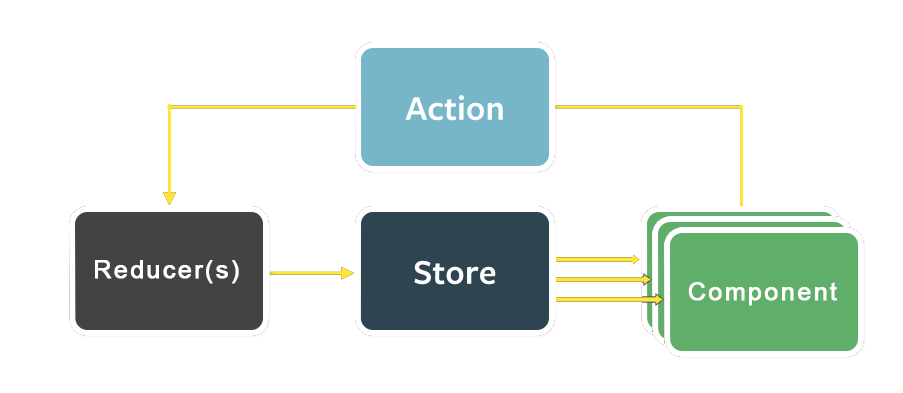
\includegraphics[scale=0.45]{main/images/redux.png}
\end{center}
\caption{Render in Redux.}
\label{fig:reduxFlow}
\end{figure}

Con Redux vengono introdotti diversi termini e concetti che è importante analizzare uno per uno.

Lo \textit{state} è quello conosciuto già in React, cioè lo stato che viene renderizzato nell'interfaccia. È buona pratica, e Redux serve proprio a questo, mantenere lo stato generale dell'applicazione nel modo più centralizzato possibile.

Le \textit{action} sono semplici oggetti JavaScript utilizzati per inviare informazioni allo \textit{store}. Si tratta dell'unico mezzo attraverso il quale si può richiedere l'aggiornamento delle informazioni presenti nello \textit{store} che è l'oggetto che mantiene lo stato dell'intera applicazione. L'unico requisito delle \textit{action} è che devono essere un oggetto contenente una proprietà \textit{type} che è la sola proprietà necessaria affinché un oggetto possa definirsi un'\textit{action}. Oltre alla proprietà \textit{type}, possiamo aggiungere altre proprietà, a seconda delle necessità e delle informazioni che vogliamo passare ai \textit{reducer}.

\lstinputlisting[style=JavaScriptStyle]{main/code/actionExample.js}

I \textit{reducer} sono le uniche funzioni autorizzate ad aggiornare le informazioni contenute nello \textit{store} il quale è l'oggetto predisposto a mantenere lo stato dell'intera applicazione.
È importante sottolineare che le funzioni \textit{reducer} non modificano l'oggetto State, ma ricevono in ingresso l'oggetto State corrente e restituiscono un nuovo oggetto \textit{state}. 
Al fine di gestire correttamente lo state centralizzato occorre creare una funzione \textit{reducer} per ogni pezzo dell'oggetto State e poi combinare tali funzioni in un unico \textit{reducer}.

\lstinputlisting[style=JavaScriptStyle]{main/code/reducerExample.js}

Lo \textit{store} è l'oggetto che mantiene lo \textit{state} dell'applicazione e fornisce alcuni metodi come \textit{getState()}, che restituisce l'oggetto \textit{state} dell'applicazione e \textit{dispatch(action)} che serve per lanciare un'\textit{action}. Lo \textit{store} ha inoltre un metodo \textit{subscribe(listener)} che serve per registrare una funzione che verrà invocata ogni volta che un'\textit{action} verrà lanciata da \textit{dispatch(action)}.

L'utilizzo della libreria Redux quindi permette di avere un oggetto unico, centralizzato a cui possono accedere più componenti contemporaneamente. Lo \textit{store} centrale e condiviso diminuisce notevolmente la complessità dei singoli componenti e riduce la duplicazione dei dati nel caso di componenti che necessitano delle medesime informazioni.

\subsection{Integrazione in OVL Dashboard}
\label{sec:integragrazione in OVL Dashboard}

Nei progetti importanti come quello trattato in questo lavoro, l'utilizzo del sistema della libreria Redux è fortemente legato al ruolo dei dati trattati all'interno del progetto. L'adozione di Redux è ottimale se l'informazione rappresentata è utile a più componenti e se serve mantenere le variabili anche dopo la distruzione dei componenti. Inoltre, nello \textit{store} Redux è possibile mantenere una sorta di cronologia delle azioni invocate. Al contrario, lo \textit{state} locale viene mantenuto per tenere traccia dei dati nel corso della vita di un certo componente, quindi da un certo punto di vista "temporanei".

La struttura dello stato in OVL Dashboard riflette quanto consigliato dalle
linee guida di Redux: un oggetto con diverse proprietà, ognuna delle quali rappresenta
una porzione dello stato indipendente dalle altre dal punto di vista logico. Queste sono:
\begin{itemize}
    \item \textit{oidc} contiene le informazioni riguardo allo stato di autenticazione dell'utente ed i dati di profilo associati ad esso (forniti dal server di autorizzazione) 
    \item \textit{invitations} contiene le informazioni riguardanti i nuovi inviti effettuati
    \item \textit{groups} contiene i gruppi delle connessioni a cui l'utente corrente ha accesso
    \item \textit{groupsConnections} contiene i gruppi e le relative connessioni a cui l'utente corrente ha accesso
    \item \textit{tickets} contiene lo stato dei ticket
\end{itemize}

Gli oggetti \textit{groups}, \textit{groupsConnections} e \textit{ticket} permettono di mantenere le rispettive informazioni fino alla chiusura della pagina in modo da effettuare il caricamento dei dati dal database solamente alla prima creazione dei componenti.

Di seguito un esempio dello stato dell'oggetto \textit{tickets}:

\lstinputlisting[style=JsonStyle]{main/code/ticketStore.json}

L'oggetto Json riportato mostra due oggetti ticket contenenti i campi riferiti allo stato e alla tipologia della richiesta e i campi necessari all'aggiunta della nuova connessione in caso il ticket venga accettato.

\section{WebRTC}
\label{sec:WebRTC}

Per la progettazione della pagina di assistenza, in particolare per l'implementazione della fase di comunicazione, si è scelto di adottare la libreria WebRTC (Real-Time Communications).
Le specifiche WebRTC nascono con l’intento di offrire agli sviluppatori web uno strumento per gestire lo scambio di flussi di dati (in primo luogo quelli multimediali come audio e video) tra due dispositivi in collegamento diretto peer-to-peer.

WebRTC offre tre API principali, utili per l'inizializzazione della comunicazione:
\begin{itemize}
    \item \textit{getUserMedia} consente di ottenere un flusso audio/video proveniente dalla telecamera e dal microfono installato sul device dell’utente 
    \item \textit{RTCPeerConnection} gestisce la connessione e la comunicazione di flussi di dati tra due dispositivi in connessione peer-to-peer
    \item \textit{RTCDataChannel} consente l’interscambio di flussi di dati arbitrari tra due dispositivi in connessione peer-to-peer
\end{itemize}

\begin{figure}
\begin{center}
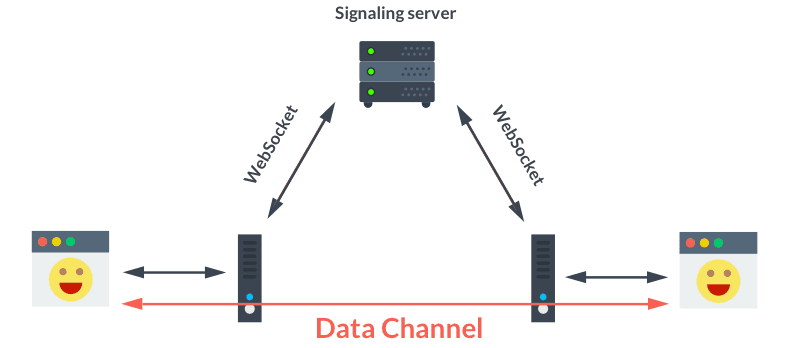
\includegraphics[scale=0.6]{main/images/WebRTC.png}
\end{center}
\caption{struttura di WebRTC.}
\label{fig:reduxFlow}
\end{figure}

Per instaurare la connessione, il sistema di WebRTC necessita in primo luogo di un signaling server. Questo server è un websocket server che permette l'interazione tra due client al fine di organizzare e impostare la comunicazione. 
Prima che due parti possano avviare una videochiamata o una chiamata, una parte deve contattare l'altra e la parte contattata deve rispondere. Questo procedimento avviene mediante un protocollo basato su offerta-risposta gestito totalmente dal signaling server.
Quando il chiamante riceve il messaggio di risposta dal ricevente, viene instaurata la connessione peer-to-peer per lo scambio di flussi di dati.

I client inizialmente si registrano presso il signaling server inviandogli un identificativo. 
La configurazione di un endpoint su una connessione WebRTC è chiamata descrizione della sessione. La descrizione include informazioni sul tipo di supporto inviato, il suo formato, il protocollo di trasferimento utilizzato, l'indirizzo IP e la porta dell'endpoint e altre informazioni necessarie per descrivere un endpoint di trasferimento multimediale. Queste informazioni vengono scambiate e archiviate utilizzando Session Description Protocol (SDP). Quando un utente avvia una chiamata WebRTC a un altro utente, viene creata una descrizione speciale chiamata offerta. Questa descrizione include tutte le informazioni sulla configurazione proposta del chiamante. Il destinatario, quindi, manda una risposta che contiene una descrizione delle informazioni sulla propria configurazione. In questo modo, entrambi i dispositivi condividono tra loro le informazioni necessarie per scambiare dati multimediali. Questo scambio viene gestito utilizzando Interactive Connectivity Establishment (ICE), un protocollo che consente a due dispositivi di utilizzare un intermediario per scambiare offerte e risposte. Ogni peer, quindi, tiene a portata di mano due descrizioni: la descrizione locale, che descrive se stessa, e la descrizione remota, che descrive l'altra estremità della chiamata.
Oltre allo scambio di informazioni sui media, i peer devono scambiarsi informazioni sulla connessione di rete. Questo è noto come candidato ICE e descrive in dettaglio i metodi disponibili che il peer è in grado di comunicare.